
\section{The Phase II Project}
\label{sec:phaseII}
%% {\em Provide an explicit, detailed description of the Phase I research
%%   approach and work to be performed.  Indicate what will be done, by
%%   whom (small business, subcontractors, research institution, or
%%   consultants), where it will be done, and how the work will be
%%   carried out.  If applicant is making a commercial or in-kind
%%   contribution to the project, please describe in detail here.  The
%%   Phase I effort should attempt to determine the technical feasibility
%%   of the proposed concept which, if successful, would provide a firm
%%   basis for the Phase II grant application.

%%   Relate the work plan to the objectives of the proposed project.
%%   Discuss the methods planned to achieve each objective or task
%%   explicitly and in detail.  This section should be a substantial
%%   portion of the total grant application.} 

\subsection{Technical Objectives}
%% {\em State the specific technical objectives of the Phase I effort,
%%   including the questions it will try to answer to determine the
%%   feasibility of the proposed approach.}

The requirements being addressed include the development of a robust framework 
for in-situ verification and validation in general purpose numerical simulation 
packages. In particular, the objective of this project is to address the need
for tools that automate verification of end-user numerical solutions in the 
NEAMS toolkit. 

In Phase II, RNET Technologies and ORNL will pursue the following objectives:

\begin{enumerate}

\item \rnetprop{Harden and extend the core VnV functionality developed during phase I. In particular, the phase II effort 
will look to determine the optimal approach for implementing the run time test injection system such that 
the risks associated with memory corruption are minimized. }
\item \rnetprop{Develop mechanisms for efficient in-situ comparisons between data in a distributed environment. In-situ comparison of variables with experimental and/or analytical results will significantly reduce the amount of IO required in \VV testing, while also providing a fine grained mechanism for detecting at what point a solution diverges from
the expected result.}
\item \rnetprop{Minimize execution times through job based parallelism. This key issue to address here 
will be to develop a mechanism for offloading tests to external processors such that the data transfer is faster than simply running the test as-is. This will shift the burden
of V\&V testing out of the main simulation, allowing for faster runtime, especially for testing methods that require the same function to be executed multiple times.}
\item \rnetprop{ Develop a robust set of generic \VV tests. The development of these tests (e.g., mesh refinement studies, the method of manufactured solutions, sensitivity analysis, uncertainty quantification) will further equip the users with the tools required to robustly perform end-user \VV.}
\item \rnetprop{Demonstrate the value of the VnV framework as a component in the NEAMS tools and into the NEAMS workbench. By showing the toolkit can be used 
in the NEAMS tools, and in particular, MOOSE, libMesh and PETSc, we will demonstrate true potential of the product in libraries that are already considered 
cutting edge across the industry. Integration into the NEAMS tools will answer the NEAMS call for tools that support end-user verification
of numerical simulations. Integration into the NEAMS workbench will provide access to the tools in the seamless manor users of the workbench have come to expect. } 

\end{enumerate}

\subsection{Work Plan}
\label{sec:workplan}

The goal of the Phase II project will be to develop a fully functional, efficient, battle tested framework 
for integrating advanced end-user verification and validation into general purpose numerical simulation packages. In what follows, we outline
the work required to satisfy the objectives outlined in the previous section and to achieve these goals. 

\subsubsection{Hardening and Optimization of the Injection Point System}

The injection point system developed during Phase I relies on C style Macros and string based type-casts. In a trusted environment, this is an efficient (void* casts are almost free) and portable (it uses low level C functionality supported by all C/C++ compilers) approach. However, there are two main weaknesses with this approach:

\begin{itemize}
 \item {\bf String based pointer casts:} The injection point system developed in Phase I requires the developer to provide a string that describes the type for each variable available at an injection point. Under the hood, the injection point system using string comparisons to ensure compatibility been test parameters and injection point variables. The key issue with this approach is that the strings specified at each injection point cannot be verified during compilation.  This will causes major issues in cases where, say, the developer changes the type of a variable, but forgets to update the type string in the injection point.  
  
 \item {\bf Restrictive type specifications:} The current system uses C compliant pre-processor macros to simplify the process of describing injection points and variables. The benefit of this approach is that the injection points can be compiled into any application without significant changes to the build system. The downside is that the single-pass, text based pre-processing supported by the C preprocessor places a significant restriction on the functionality that can be imparted.
\end{itemize}
 
In Phase II, the project team will investigate and develop an annotation based system for defining injection points. This annotation system will be far more dynamic, allowing users to full control over what variables can be accessed at each injection point, including the ability to provide access to internal components of data structures, describe the domain decomposition of distributed arrays and to complete pre-test processing of variables. The annotation system will also provide a mechanism for suggesting default tests to be run at each injection point, and will provide a mechanism for injection point detection in non-object orientated programming languages where runtime injection point detection cannot be completed. However, the primary benefit of this new system will be that it will automatically detect the type of the variables tagged for inspection at each injection point.  

To implement this annotation system, the project team will create a set of custom pre-processor directives (i.e., pragmas) using Clang. Clang is a compiler front end for the C family of languages. It is a well supported, well documented compiler package designed as a drop in replacement for GCC. In particular, Clangs simple API for defining custom Pragma routines, combined with its robust API for walking the Abstract syntax tree of the code make it the perfect choice for developing this system. Clang has seen wide scale uptake across the software development world and, in recent years, has emerged as a realistic competitor to the ubiquitous GCC compiler suite.  

\subsubsection{Efficient Statistical Comparisons in Distributed Settings} 

One of the major benefits of the VnV framework is that it allows for in-situ testing and analysis in distributed systems. In particular, this type of in-situ analysis is particularly useful for analyzing and comparing data stored in distributed arrays. For example, VnV tests could be used to assert that all the elements in an array are positive, or that all the elements in an array are the same as the elements in another array within some tolerance. From the perspective of \VV, such tests would allow for in-situ comparisons with experimental data and for fine-grained regression testing. To that end, a large portion of the Phase II project will be devoted to developing efficient methods for analyzing, asserting and comparing data stored in distributed arrays. 

Some information about the global distribution of the data is needed to act of distributed data. Determining this global partition is not difficult for programs that use a regular decomposition scheme because, in these cases, there exists a static o(1) mapping function that can be evaluated locally on any processor to determine the owner of any index. For irregular decompositions, where no such function exists, some form of intra-processor communication is needed to form the global partition. 

The naive approach to determining the data partition is to explicitly form the global partition using global MPI communication. This is a robust approach that will be immediately applicable in a large number of situations. However, the large storage cost required to build the global partition (O(P), where $P$ is the number of processors) is likely to become an issue in peta- and exa-scale environments \cite{hypre-assumed}. 

To that end, the Phase II effort will include a detailed analysis of the optimal algorithms for forming the global partition in a distributed setting. This will include the implementation and profiling of the aforementioned naive approach, as well as an investigation into more advanced approaches such as forming a hash based distributed directory \cite{hpre-nine} and the assumed partition algorithm \cite{hypre-assumed}. 

Once the intra-processor communication patterns have been determined, the focus will shift to developing efficient algorithms for comparing and analyzing distributed data. This will include the development of the VnV Testing suite for distributed Arrays. This testing suite will include a variety of analysis routines for analyzing data including, means, std deviation, variance, co-variance, etc. A collection of functions implementing matrix based metrics will also be included (e.g., one norms, symmetry, positive definiteness, etc). 
In each case, these analysis routines will be implemented in a distributed manor than minimizes intra-processor communication. Moreover, rather than being implemented as a independent functions, all analysis routines will be completed simultaneously, minimizing memory accesses and further reducing communication overheads. 

The testing suite will also include several tools for comparing data stored in distributed arrays with data stored on file and data in other arrays. Such functionality will
be particularly useful when comparing test solutions with experimental or expected results. It will also be useful for regression testing as it provides a fine grained mechanism
for detecting the exact point at which a simulation moves away from the expected solution. 

The naive approach to comparing distributed arrays would be to collect the data on some home processor for analysis. However, in a high performance setting, this is not a feasible approach, both because of this high communication costs and because, in many cases, the arrays are simply to large to fit in the memory of a single core. Hence, there is a strict requirement that the comparison be completed in a distributed fashion. 



\subsubsection{Reducing Run-times with Test Offloading and Job Parallelism}

Performing a large number of \VV tests in a distributed environment will be expensive, both computationally and due to the data movement required to deal with the domain decomposition employed by the application. 

To address this problem, the VnV toolkit will have built in support for offloading tests to external processes. This functionality will allow for speedup through job parallelism for expensive testing routines like sensitivity analysis and mesh refinement, while also allowing for specific tests to be run on the optimal architecture (e.g., an test involving image processing could be offloaded to a GPU enabled architecture).  

The first step toward supporting test offloading will be to implement an effective mechanism for transferring the required 
data from the simulation to the external testing processes. To do this, the project team will use the ADIOS 2 Sustainable Staging Transport (SST). The SST is a classic streaming data architecture that allows for direct connection between data produces and data consumers via the ADIOS2 write/read API. In HPC environments, SST uses the RDMA interconnects to ensure fast transfer of data between HPC applications; however, socket based connections are also supported. 

The VnV toolkit will use the SST engine to distribute the required testing data to a VnV Testing Manager. The role of the test manager will be to determine, based on the data provided, the best available resource for running the given test and to launch the required executables. The test manager will be a C++ executable that makes use of the Eclipse Parallel tools platform (PTP). The PTP project provides an integrated development environment to support the development of parallel applications written in C, C++, and Fortran. Eclipse PTP provides; support for the MPI, OpenMP and UPC programming models, as well support for a wide range of batch systems and runtime systems, including PBS/Torque, LoadLeveler, GridEngine, Parallel Environment, Open MPI, and MPICH2. In this case, the test manager will use the PTP platforms extensive support for integrating with remote job schedulers to launch tests on the best available resource. 

The final step toward test offloading will be to develop the infrastructure required to launch tests as separate, independent executables capable of consuming data using the ADIOS2 API.   

\subsubsection{Integrate Third Party Tools for Mesh Refinement, UQ and Sensitivity Analysis.}

Mesh refinement studies, uncertainty quantification and sensitivity analysis are all essential components of a robust \VV regimen. To that
end, the Phase II effort will include the development of \VV tests that integrate third party tools to complete these tests. 

The UQ and SA tests will be developed using DAKOTA. DAKOTA provides a set of black-box tools for performing parameter optimization, UQ 
and SA. DAKOTA provides two interfaces for integrating these tools into applications; a black-box approach that uses preprocessors, post-processors
and the file system to complete the tests; and a library API for direct, hard-coded testing. The Phase II 
effort will include the development of an custom VnV testing library for direct integration with the DAKOTA library API. This will include the development
of a flexible interface for setting up and running the DAKOTA tests, and the development of the test specification files for displaying the test results 
in an informative and interactive way. 

Support for Mesh refinement will be developed as part a separate plug-able VnV testing library. The intended functionality of this testing 
suite will be to enable the completion of both uniform and adaptive mesh refinement studies given only the initial coarse mesh. This will require 
the development of methods for marking the mesh for refinement and methods for refining the mesh. Most high performance finite element packages support
some level of adaptive mesh refinement (e.g., libMesh, Fenics, MFEM, etc.), hence, rather than trying to patch in third party tools, the mesh-refinement tool 
will be developed as a generic interface for interacting with existing mesh refinement functionality. 

An additional test for tracking and displaying a detailed provenance history for the simulation will also be developed. This provenance tracking
test will be attached to the main function of the executable and will include functionality for documenting the inputs to the code, the build 
date of the executable, a list of the versions, checksums and build dates of any imported shared libraries, copies of the stdout, stdin and stderr, and, where 
appropriate, copies of all output files. Tracking these details is not difficult, yet, this detailed level of information will significantly increase the validity of the \VV report while also providing a mechanism for detecting when a \VV report becomes out of date due to an upstream software update. 

\subsubsection{Integration with NEAMS tools and the NEAMS workbench} 

The next step in the Phase II project will be to integrate the VnV framework into the NEAMS 
tools. Doing so will provide ample opportunities for testing, while also allowing us to demonstrate the performance of the toolkit in real codes with
real applications. Moreover, this integration will answer the solicitations call for tools that support end-user verification of numerical solutions in the NEAMS tools. 

Integration into NEAMS tools will be a three step process:

\begin{itemize}
 \item The first step will be to insert injection points into key locations in the MOOSE, libMesh and PETSc source codes. The optimal locations for 
 inserting these injection points will be determined after detailed profiling of example codes; however, some obvious options include during each linear 
 solver iteration, during each nonlinear iteration, during finite element matrix construction (if it exists) and inside the function for calculating the action of the Jacobian
 on a vector. The project team demonstrated the ability to insert injection points into MOOSE code during Phase I (see Section~\ref{sec:feasibility}. 
 
 \item The second step will be to allow users to configure the VnV testing directly in the MOOSE input file using the MOOSE input
file syntax. This will provide users of MOOSE with a seamless mechanism for setting up and running tests. This will be completed by
developing a custom MOOSE ``Action'' that sets up the core VnV testing functionality. 
\item The third step will be to enable context-aware auto-complete for MOOSE based VnV configuration files in the NEAMS workbench. The workbench
has integrated support for extracting the information required to setup input file verification and auto-complete from MOOSE applications; however, there
will likely be some additional work required to correctly setup the auto-complete and verification for tests stored in external libraries. In particular, the current system 
requires that the tests adhere to a specific XSD specification, but there is not yet a system for extracting the exact parameters required to inject a specific test. To do this, we will create a lightweight executable that loads external test libraries and extracts the appropriate parameter specifications in the ``SON'' format supported by workbench.  
\item The last step will be the development of an interface for editing the YAML specification files used to generate the final report and an interface 
for viewing the final reports. The GUI will be written using standard HTML and Javascript and then integrated into the workbench using the QT QWebEngineView component. The QWebEngineView component allows for interactions with the core QT window (i.e., open, save, copy, paste, etc.) however, it is important to note that this approach will not allow for a truly ``native'' experience within the workbench. The decision to develop in JS and HTML rather than native QT was made to ensure the final product, the VnV framework, is consistent, and can be used in applications outside of the NEAMS lines of tools. Every effort will be made to ensure the GUI conforms to the NEAMS workbench standards and specifications. 
\end{itemize}

\subsubsection{Preparation for First Release} 

The final step in the Phase II project will be to complete the miscellaneous tasks required to prepare 
the toolkit for production. \. This will include:
\begin{itemize} 
 \item Adding support for a wider range of data visualization techniques. As shown in the feasibility section, the Phase I prototype supports some 2D plots and 3D plotting of .VTP files. In Phase II we will extend this support to include a wide range of charts and a wide range of VTK file formats. In addition, the project team will add support for rendering 3D plots using an instance of Paraview running on the local machine of the user who is reading the report. This functionality, which is already supported by ParaviewWeb, will allow for more detailed visualizations that can be implemented with static data and post-processing alone. 
 \item Adding support for the industry specified \VV report Templates, such as the DoD \VV template specification \cite{}. This functionality will furter increase the value of toolkit in industry settings where specific formats a required for \VV reporting. 
 \item Hardening the build system, finalizing documentation, writing user manuals and creating tutorials.
 

 \end{itemize}


\subsection{Performance Schedule and Task Plan}
\label{sec:taskplan}

% Use wrapfigure here instead?
\begin{wrapfigure}{r}{0.5\linewidth}%[thb]
%\begin{figure}[thb]
\begin{center}
\leavevmode
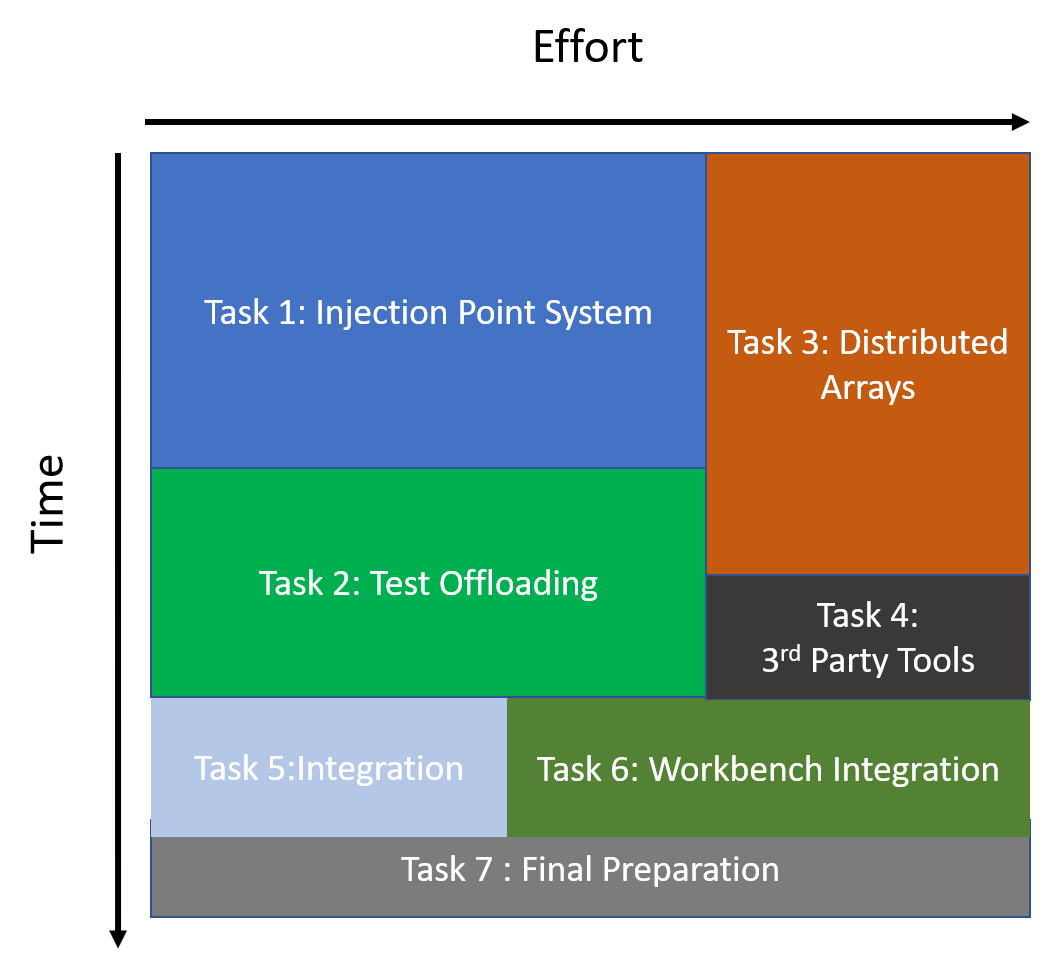
\includegraphics[width=1.0\linewidth]{./narrative/figures/tasks.png}
\end{center}
\caption{Overview of task dependencies and timeline.}
\label{fig:tasks}
\end{wrapfigure}

RNET would like to present the project ideas and research plan to the
DOE Program Manager and other interested scientists. The meeting will
be used to discuss features, and identify the specific NEAMS applications and computer
resources that will benefit from this project.  This meeting will be
scheduled soon after the Phase II contract is awarded. The meeting can
be hosted at RNET, a DOE site suggested by the Program Manager or via
a teleconference.

RNET will submit all reports as required by the contract (e.g., annual reports, 
a continuation report, summary reports, and a final report) to the DOE program 
manager and other interested DOE scientists.

The research and development topics described in Section~\ref{sec:workplan} 
will be addressed by the tasks described in the remainder of this section. Most 
tasks require active collaboration between RNET and its collaborators. 
Figure~\ref{fig:tasks} summarizes at a high level the dependencies among tasks  and
approximate anticipated task durations. The duration of the Phase II 
project is 104 weeks. Specific details are included in the description of each 
task.


\newcounter{taskCount}
\setcounter{taskCount}{0}

\refstepcounter{taskCount}\label{task:2.5}
\subsubsection{Task \ref{task:2.5}: Development of the Annotation based Injection Point System  }

In this task, the project team will develop the Annotation system for specifying injection points and describing injection variables. This will include the development of
the custom LLVM compiler extensions required to process these annotations. At the end of this task, users will be able to specify injection points and injection variables using either the new Annotation point system, or using the more portable, but less robust Phase I approach. 

To test the Annotation based injection point system, the project team will write injection points at several key locations in the MOOSE software stack, including inside the source code of several MOOSE modules, the core MOOSE framework, libMesh and PETSc. This will allow us to demonstrate the cross-library potential of the Annotation based system, while also acting as the first step toward integration of the tools a number of the NEAMS tools. 

\rnetprop{RNET will work on the implementation for this task and ORNL will provide inputs and guidance.}


\refstepcounter{taskCount}\label{task:3}
\subsubsection{Task \ref{task:3}: Develop methods for offloading tests to external processes. }

In this task, the project team will add support for test offloading using the ADIOS2 SST architecture. This will include 
the development of the VnV test manager and integration with the PTP platform, a task which will likely involve custom modifications
to the PTP platform. Once implemented, test offloading will be tested using the VnV enabled MOOSE software stack developed in Task~\ref{task2.5}. The 
goal of this task will be to see a 5x speedup when using test offloading over the standard in-situ testing routines. 

\rnetprop{RNET will work on the implementation for this task with ORNL providing assistance with any modifications to PTP. }

\refstepcounter{taskCount}\label{task:23}
\subsubsection{Task \ref{task:23}: Development of efficient statistical \VV tools for distributed arrays.}

In this task, the project team will investigate the optimal approaches for conveying information about the data decompoosition to the individual tests. This will involve robust analysis of the three aforementioned approaches to determining the global partition; explicitly forming the global partition; building a distributed directory; and using an assumed partition algorithm. This task will also include the development of a number of efficient statistical tools for asserting the state of the data in distributed arrays.

At the completion of this task, users will be able to efficiently compare and analyze distributed arrays using the VnV framework. To test these implementations, the project team will set up tests for performing assertions on various PETSc vectors and matrices. This testing will compare the performance of each of the global partition methods and each of the analysis tools. 

\rnetprop{RNET and ORNL will collaborate on this task.}

\refstepcounter{taskCount}\label{task:22}
\subsubsection{Task \ref{task:22}: Development of Generic tools for Mesh refinement, Uncertainty quantification and Sensitivity Analysis.}
In this task, RNET will implement generic \VV tools for mesh refinement, uncertainty quantification and sensitivity analysis. In the case of mesh refinement, the approach taken will be to create a generic interface for interacting with the automatic mesh refinement functionality that already exists in finite element libraries like LibMesh and Fenics. The overall goal is to create a generic VnV test that can be attached to the main function of the executable such that it automates the process of running mesh refinement and mesh convergence studies. In the case of UQ and SA, the project team will develop an interface for specifying the tools available in DAKOTA as VnV tests. 

\rnetprop{RNET will be responsible for this task with ORNL providing input and guidance. }


\refstepcounter{taskCount}\label{task:1}
\subsubsection{Task \ref{task:1}: Integration into real applications, including the NEAMS Tools}
\rnetprop{
  In this task, the program team will integrate the VnV framework into a variety of real applications. Initially, this 
  testing will be completed in tools used heavily in the NEAMS toolkit; MOOSE, libMesh and PETSc, but other third party 
  applications will also be investigated. To ensure seamless integration with the MOOSE tools, the project team will reimplement
  the XML based configuration file using the MOOSE input file format. This will allow for the configuration of the VnV tests in 
  a MOOSE application directly from the input file.
  
  The goal of this task will be to generate informative, production quality VnV 
  reports for a number of examples available in the MOOSE testing suite. Doing so allows us
  to test every facet of the proposed framework, while also acting the first demonstration of the
  value provided by the framework. These results of these tests will be hosted on the RNET website 
  as they become available. 
 

}

\rnetprop{
RNET will be responsible for this task and ORNL will provide guidance on 
various technical implementations and details.
}
\refstepcounter{taskCount}\label{task:11}
\subsubsection{Task \ref{task:11}: Development of an interface for the NEAMS workbench}
\rnetprop{
  In this task, the project team will integrate the toolkit directly into the NEAMS workbench. This will be
  a two stage process. First, the project team will implement the required interface files for enabling 
  the context aware auto-complete features available in the NEAMS workbench for the MOOSE based configuration
  file specification developed in the previous section. MOOSE based input files are already largely supported in
  the workbench; however, there will likely be some issues with determining which tests are applicable at which 
  injection points. Second will be developing an interface for customizing and viewing the final VV report. As part of the Phase I
  effort, the project team demonstrated viewing the final \VV report in a QT WebView component. The workbench is also but on to
  off QT, hence we do not expect to many difficulties on that front. Instead the key objective will be to develop the mechanisms for
  displaying customizations made the the final report in real-time within the NEAMS workbench. 
}
\rnetprop{ RNET will be responsible for this task }


\refstepcounter{taskCount}\label{task:4}
\subsubsection{Task \ref{task:4}: Preparation for the First Release }
In this task, the project team will prepare the package for its first release. This will include writing documentation (user manuals, tutorials, etc.), extending 
the custom VnV markdown specification and adding support for generating reports that conform to industry specific standards. 

\rnetprop{RNET will work on the implementation for this task}


\subsection{Facilities/Equipment}
\subsubsection{RNET Facilities}
RNET has the necessary office equipment to manage an SBIR/STTR contract
including networks, workstations, and accounting software. In
addition, RNET has the tools (software and hardware) to evaluate and
develop the technologies proposed here.  

RNET currently has 9 development computers and a 10-node development cluster 
that can be used for development and testing in this effort. Each cluster node 
has two quad-core or hexa-core XEON CPUs, 24-32GB of DRAM, 500+GB of local 
disk. 
Two data networks are available, a COTS 1 Gbps Ethernet network and a 10 Gbps 
Ethernet network. The Linux development nodes and the RNET cluster have the 
necessary Linux/GNU toolchains and development environments including; GNU 
tool chain, Microsoft .Net Framework, and Java Standard Edition.

\subsubsection{ORNL Facilities}
%\rnetcomment{Jay to verify, can we state these resources can be used on this project?}
The Oak Ridge National Laboratory (ORNL) hosts three petascale computing 
facilities: the Oak Ridge Leadership Computing 
Facility (OLCF), managed for DOE; the National Institute for Computational 
Sciences (NICS) computing facility operated 
for the National Science Foundation (NSF); and the National Climate-Computing 
Research Center (NCRC), formed as 
collaboration between ORNL and the National Oceanographic and Atmospheric 
Administration (NOAA) to explore a variety of 
research topics in climate sciences. Each of these facilities has a 
professional, experienced operational and engineering 
staff comprising groups in high-performance computing (HPC) operations, 
technology integration, user services, scientific 
computing, and application performance tools.

ORNL also has the Compute and Data Environment for Science (CADES) which is a 
fully integrated infrastructure offering compute and data services for 
researchers lab-wide. We will work with appropriate program managers to apply 
for allocation requests as appropriate.


 The ORNL computer facility staff 
provides continuous operation of the centers 
and immediate problem resolution. On evenings and weekends, operators provide 
first-line problem resolution for users with 
additional user support and system administrators on-call for more difficult 
problems. ORNL also has state-of-the-art 
visualization facilities that can be used on site or accessed remotely. 
